\documentclass{standalone}
\usepackage{tikz}
\usepackage{ctex,siunitx}
\usepackage{tkz-euclide}
\usepackage{amsmath}
\usetikzlibrary{patterns, calc}
\usetikzlibrary {decorations.pathmorphing, decorations.pathreplacing, decorations.shapes,}
\begin{document}
\small
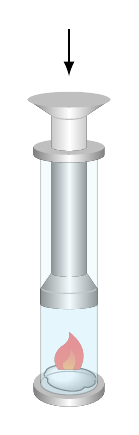
\begin{tikzpicture}[>=latex,xscale=1.5]
  \fill[left color=gray,right color=gray,middle color=white](-0.3,0)--++(0,-0.1)arc(180:360:0.3 and 0.2)--++(0,0.1)--cycle;
  \fill[lightgray](0,0)ellipse(.3 and 0.2);
  \draw[ball color=white](-0.2,0.14)to[bend left=80](0.05,0.17)to[bend left=80](0.22,0.03)to[bend left=80](0.13,-0.05)to[bend left=90](-0.18,0.06)to[bend left=60]cycle;
  \fill[top color=red,bottom color =red!80!orange](-0.09,0.17)to[bend left](-0.07,0.46)to[bend right](0,0.65)to[bend left](0.09,0.17);
  \fill[top color=red!90,bottom color =orange](-0.03,0.17)to[bend left](-0.05,0.26)to[bend right](0,0.45)to[bend left](0.03,0.17);
  \draw[gray](-0.24,0)arc(180:0:0.24 and 0.15);
  \fill[cyan!15,opacity=0.5](-0.24,0)arc(180:360:0.24 and 0.15)--++(0,1)--++(-0.48,0)--cycle;
  \fill[left color=gray,right color=gray,middle color=white](-0.24,1)arc(180:360:0.24 and 0.06)--++(0,0.2)--++(-0.09,0.2)--++(-0.3,0)--++(-0.09,-0.2)--cycle;
  \fill[lightgray](0,1.4)ellipse(.15 and 0.05);
  \fill[left color=gray,right color=gray,middle color=white](-0.15,1.4)arc(180:360:0.15 and 0.05)--++(0,1.6)--++(-0.3,0)--cycle;
  \draw[lightgray](-0.23,1.2)arc(180:360:0.23 and 0.06);
  \fill[cyan!20,opacity=0.2,draw=black](-0.24,0)arc(180:360:0.24 and 0.15)--++(0,3)--++(-0.48,0)--cycle;
  \fill[left color=gray,right color=gray,middle color=white](-0.3,3)--++(0,-0.1)arc(180:360:0.3 and 0.1)--++(0,0.1)--cycle;
  \fill[lightgray](0,3)ellipse(.3 and 0.1);
  \fill[left color=gray,right color=gray,middle color=white](-0.15,3.0)arc(180:360:0.15 and 0.05)--++(0,0.4)--++(0.2,0.2)--++(-0.7,0)--++(0.2,-0.2)--cycle;
  \fill[lightgray](0,3.6)ellipse(.35 and 0.1);
  \draw[lightgray](-0.14,3.4)arc(180:360:0.14 and 0.05);
  \draw[thick,->](0,4.5)--(0,3.9);
\end{tikzpicture}
\end{document}